\section{Magnitude Estimation Relevance Judgments}
\label{sec-rq1}

Having obtained magnitude estimation scores for 4,269 topic-document
pairs, we analyze the user-perceived relevance to answer the first
research question RQ\ref{item:rq1}, whether the magnitude estimation
technique is suitable for gathering document level relevance
judgments, and whether the resulting relevance scales are reasonable
with respect to our current knowledge of relevance judgments.

% \subsection{Consistency of Magnitude Estimation and Ordinal Relevance}
% \label{sec:cons-magn-estim}

\begin{figure}[t]
  \centering
  \includegraphics[width=.7\linewidth,page=19]{figs/check_gross_ranks_med.pdf}
  \vspace{-0.5cm}
  \caption{ME score distribution by Sormunen and TREC levels.}
  \label{fig:ME-distribution}
\end{figure}


\begin{figure}[tp]
  \centering
  %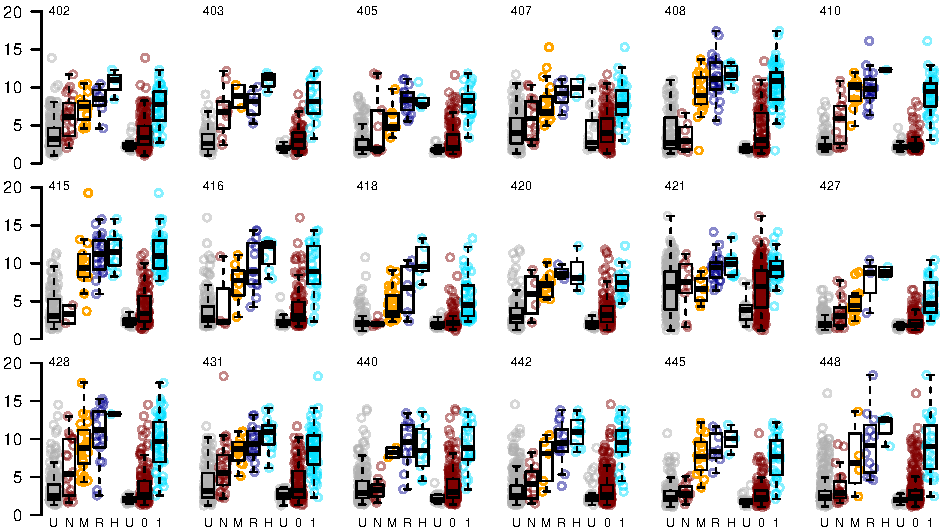
\includegraphics[angle=90,height=.9\textheight,page=1]{figs/check_gross_ranks_med_all.pdf}
  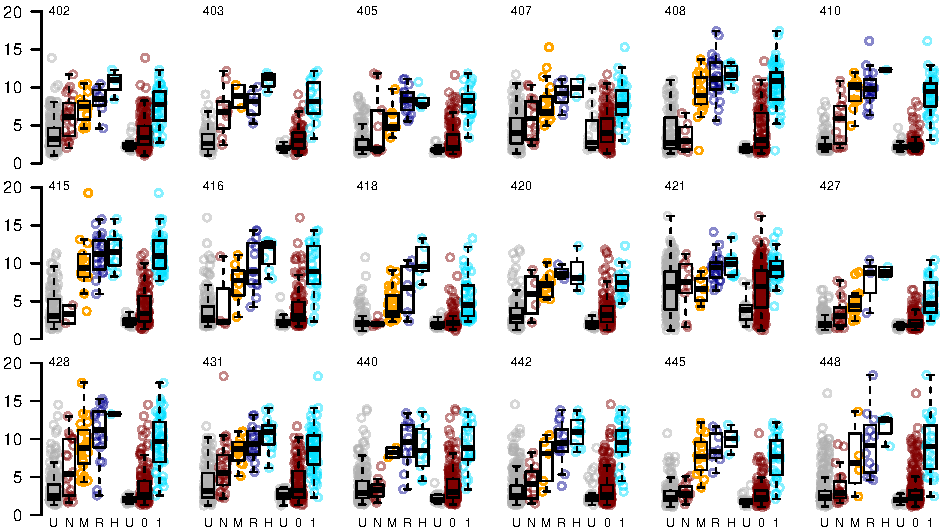
\includegraphics[width=\linewidth,page=1]{figs/check_gross_ranks_med_all.pdf} %
  \caption{ME score distribution by Sormunen (U, N, M, R, H) and TREC (U, 0, 1) levels:
    breakdown for individual topics.
  \label{fig:ME-distribution-breakdown}
   }
\end{figure}

The distribution of the median normalized magnitude estimation scores
for each document are shown in Figure~\ref{fig:ME-distribution},
aggregated across all 18 topics, and split by Sormunen ordinal
relevance levels (left side of figure, levels are 
\nn, \mm, \rr, \hh, and {\tt U}, the group of documents that were not judged
by Sormunen), and by TREC binary levels (right side of figure, levels
are $0$, $1$, and {\tt U}, the documents that were not judged by TREC,
as not all participating runs were included in the judging pool).
Boxplots in this paper show the median as a solid black line; boxes
show the 25th to 75th percentile; whiskers show the range, up to 1.5
times the inter-quartile range; and outliers beyond this range are
shown as individual points.

There is a clear distinction between each of the four adjacent Sormunen
levels (two-tailed t-test, $p<0.002$), with the magnitude estimation
scores on average following the ordinal scale rank ordering.
The differences between the two TREC levels are also significant
($p<0.001$), with the magnitude estimation scores on average again
being aligned with the binary levels.
This is strong evidence for the overall validity of the magnitude
estimation approach.

Figure~\ref{fig:ME-distribution-breakdown} shows the magnitude
estimation score distributions for each of the 18 individual topics.
Although there is some variability across topics, overall the figure
confirms that the magnitude estimation scores are generally aligned
with ordinal categories even when considering individual topics: the
medians of the median magnitude estimation scores (the solid black
lines) generally follow the ordinal categories, for all categories and
for all topics (there are a small number of exceptions for some of the
Sormunen adjacent categories in topics 403, 405, 410, 420, 421, and
440; there are no exceptions for non-adjacent categories, nor for TREC
categories).
Since for each topic there could potentially be 3 exceptions for
adjacent categories, and 6 exceptions in general, plus one exception
for the two TREC categories, the 6 exceptions found are out of $3 * 18
+ 18 = 72$ possible cases when considering only adjacent categories, or
out of $6 * 18 + 18 = 126$ cases when considering also non-adjacent
categories.
Such a limited fraction of exceptions (in the $5\%$-$8\%$ range) is
further strong evidence for the validity of our approach, even at the
single topic level.

Regarding the set of documents that were not judged by Sormunen
(left-most boxes in Figure~\ref{fig:ME-distribution} and sub-plots in
Figure~\ref{fig:ME-distribution-breakdown}), based on the magnitude
estimation scores it can be inferred that the bulk of this class are
likely to be non-relevant; however there are also instances that occur
across the central parts of the marginal to highly relevant score
distributions. There were also a handful of documents unjudged by 
TREC that seemed to be rated highly by our judges.
While the overall distributions of
magnitude estimation scores are strongly consistent with the ordinal
and binary categories, there are also documents in each class 
where the ME scores 
fall into the central region of a different class.


% \subsection{Judge Agreement}
% \label{sec:judge-agreement}


% Local Variables:
% TeX-master: "ME-TOIS.tex"
% End:
